\documentclass[12pt]{article}
\usepackage{amssymb,amsmath,amsthm}
\usepackage{expdlist}  % or fancyvrb depending on your editor’s support
\usepackage{float}
\usepackage{graphicx}
\usepackage{booktabs}
\usepackage{tikz}
\usepackage{color}
\usepackage{listings}
\usepackage{xcolor}
\definecolor{lightblue}{RGB}{173, 216, 230}
\definecolor{dkgreen}{rgb}{0,0.6,0}
\definecolor{gray}{rgb}{0.5,0.5,0.5}
\definecolor{mauve}{rgb}{0.58,0,0.82}
\lstset{frame=tb,
  language=Python,
  aboveskip=3mm,
  belowskip=3mm,
  showstringspaces=false,
  columns=flexible,
  basicstyle={\small\ttfamily},
  numbers=left,
  numberstyle=\tiny\color{gray},
  keywordstyle=\color{blue},
  commentstyle=\color{dkgreen},
  stringstyle=\color{mauve},
  breaklines=true,
  breakatwhitespace=true,
  tabsize=3
}

% define command \expandableinput  for table input
\makeatletter
\def\expinput#1{\@@input#1 }
\makeatother 

\begin{document}

% Display title
\begin{titlepage}
  \centering
  \vspace*{1in}
  \huge
  \textbf{Parallelization of 2D Finite Difference Schemes with UNM CARC Super Computer Network}\\[0.5in]
  \Large
  \textbf{Author:}\\[0.2in]
  Tanner Wagner\\[1in]
  \normalsize
  \today
  \vfill
\end{titlepage}

\newpage
\tableofcontents
\newpage


\section{Overview}
The goal of this assignment is to develop and implement a 2D finite difference method to compute some numerical derivatives. We are then interested in measuring the size of the error $e$ of this numerical approximation to the derivative. This means that we will compute the integral of the difference between the exact derivative (which I have calculated on my own) and the approximate numerical derivative. In doing this, we will explore the use for UNM's CARC super-computer and the technique of parallelization to better represent our data.

\section{Mathematical Foundations}
\subsection{Derivation of the Finite Difference Method}
To approximate the second derivatives, we use the $\textit{central difference method}$, derived using the Taylor expansion.
\\
\\
For a grid point \( u_{i,j} \), the Taylor expansions of neighboring points are:
\begin{align*}
    u(x+h, y) &= u(x,y) + h u_x + \frac{h^2}{2} u_{xx} + \mathcal{O}(h^3), \\
    u(x-h, y) &= u(x,y) - h u_x + \frac{h^2}{2} u_{xx} + \mathcal{O}(h^3).
\end{align*}
\noindent Adding these two equations gives:
\[
    u_{xx} \approx \frac{u_{i+1,j} - 2u_{i,j} + u_{i-1,j}}{h^2} + \mathcal{O}(h^2).
\]
\\
\noindent A similar derivation holds for the \( y \)-direction, resulting in:
\[
    u_{yy} \approx \frac{u_{i,j+1} - 2u_{i,j} + u_{i,j-1}}{h^2} + \mathcal{O}(h^2).
\]
\\
\noindent Combining these, the **discrete Laplacian** operator becomes:
\[
    \nabla^2 u \approx \frac{u_{i+1,j} + u_{i-1,j} + u_{i,j+1} + u_{i,j-1} - 4u_{i,j}}{h^2}.
\]
\\
\noindent This is implemented using the following **five-point stencil**:
\[
\frac{1}{h^2}\begin{bmatrix} 0 & 1 & 0 \\ 1 & -4 & 1 \\ 0 & 1 & 0 \end{bmatrix}.
\]

\subsection{Error Analysis and Accuracy}
The truncation error for this method is **second-order accurate**, meaning:
\[
    \text{Error} \sim \mathcal{O}(h^2).
\]
\\
\noindent To verify this, the \( L_2 \)-norm of the error \( e \) is computed:
\[
\lVert e \rVert_{L_2}  := \left( \int_{[0,1] \times [0,1]} (u_{xx}^{\text{approx}} - u_{xx}^{\text{exact}})^2 + (u_{yy}^{\text{approx}} - u_{yy}^{\text{exact}})^2 \; dx \; dy \right)^{1/2}.
\]



\subsection{Problem Description}
We are asked to consider the function
\[
u(x,y) = \cos((x+1)^{1/3}+(y+1)^{1/3})+\sin((x+1)^{1/3}+(y+1)^{1/3})
\]
\noindent over the unit square $\Omega := (x,y) \in [0,1] \times [0,1]$.
\\
\\
We will assume the number of grid points in each dimension to be the same and we will denote this number of grid points as $n$ such that the grid spacing is given by
\[
h = \frac{1}{(n-1)}.
\]
\\
\noindent Thus, we have a total of $n^2$ grid points with $n$ points in the $x$-direction and $n$ points in the $y$-direction.
\\
\\
We then want to notice that the Dirchlet boundary condition $g(x,y)$ is defined as $u(x,y)$ on the boundary s.t.
\[
g(x,y) = \cos((x+1)^{1/3}+(y+1)^{1/3})+\sin((x+1)^{1/3}+(y+1)^{1/3}),
\]
\noindent $\forall (x,y) \in \partial \Omega$, where $\partial \Omega := \{(x,y) \text{ such that }  x = \{0,1\} \text{ or } y = \{0,1\}\}$.
\\
\\
\noindent What we want to do next is to compute the integral of the difference between the exact derivative and the approximate numerical derivative which is given as the $L_2$ norm of $e$ which is given by
\[
\lVert e \rVert_{L_2}  := \left( \int_{[0,1] \times [0,1]} \left( \frac{\partial^2 u}{\partial x^2} \bigg|_{\text{approx}} - \frac{\partial^2 u}{\partial x^2} \bigg|_{\text{exact}} 
+ \frac{\partial^2 u}{\partial y^2} \bigg|_{\text{approx}} - \frac{\partial^2 u}{\partial y^2} \bigg|_{\text{exact}} \right)^2 \, dx \, dy \right)^{1/2}
\]  

\section{Implementation in Serial with Error Analysis}
\subsection{What}
We are given that the finite difference stencil used for approximating the second derivative is given by the matrix product
\[
\frac{1}{h^2}\begin{bmatrix} 0 & 1 & 0 \\ 1 & -4 & 1 \\ 0 & 1 & 0 \end{bmatrix}
\]
\\
\noindent We then want to use the provided .py file poissson.py (which contains the function poisson()) to generate the CSR matrix that cotains the finite difference stencil.

\subsection{How}
To solve this problem, I considered the TODOS in the skeleton code and first checked this for numthreads = 1. I saw that my outputs were all evenly represented and printed $0$ with the helper function checkmatvec; which was provided. Finally, provided below are log-log plots that demonstrate that the numerical solution converges quadratically which is to be expected given the definition of the second-order accuracy of the finite differece method. In this first problem, we are only interested in 1 thread; which the plot displays.

\begin{figure}[H]
    \centering
    \includegraphics[width=0.5\textwidth]{error1.png}
    \caption{log-log Plot of Error VS. Grid Size for Serial Implementation.}
\end{figure}


\subsection{Why} 
What the output of hw4skeleton really shows is how the boundary conditions and the finite difference stencil actually work to effect the matrices sparsity. This output isn't too helpful for the report since its output in text can be convoluted, but can be seen by running the code for yourself. What the report is really showing in this section is that we computed the $L_2$  norm of $e$ and the figure generated shows that the numerical solution is converging quadratically given our reference plot which is consistent with the second-order finite difference method. 

\section{Implementing in Parallel with CARC Performance Analysis}
\subsection{What}
What we are interested in doing this next section is showing the performance that was captured both on my local machine as well as the CARC platform. What we should see is that my parallelized code yields the same results as my serial code for threads 1-3.

\subsection{Subdomain Splitting and Halo Regions}
To parallelize the 2D finite difference scheme, the computational grid is split into $\textit{subdomains}$, one for each thread. Each subdomain contains **halo regions** (ghost cells) to communicate boundary values between neighboring subdomains.










\begin{figure}[H]
  \centering
  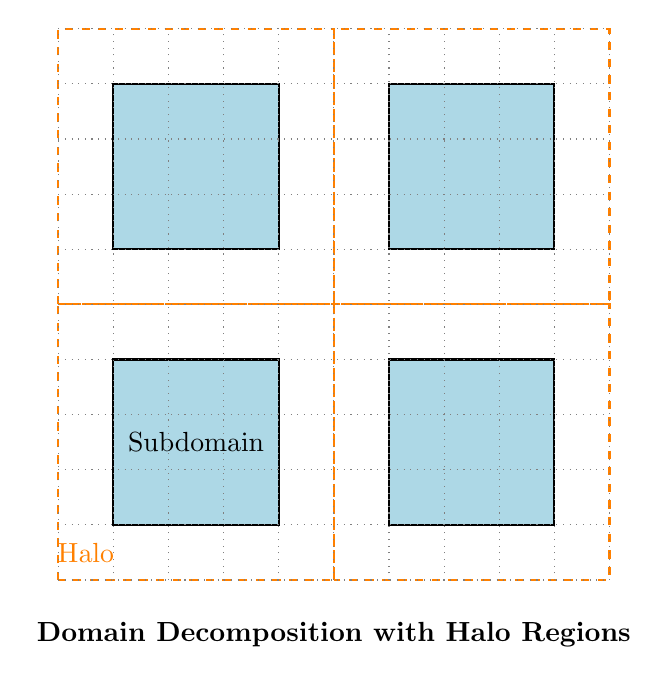
\begin{tikzpicture}[scale=0.7]
    % Parameters
        \def\n{5} % Grid size per subdomain including halos
        \def\s{2} % Number of subdomains

        % Draw subdomains and halos
        \foreach \i in {0,1} {
            \foreach \j in {0,1} {
                % Halo Region (Outer)
              \draw[thick, dashed, orange] (\i*\n, \j*\n) rectangle ++(\n, \n);

              % Subdomain Interior (Inner)
                \fill[lightblue] (\i*\n+1, \j*\n+1) rectangle ++(\n-2, \n-2);
                \draw[thick] (\i*\n+1, \j*\n+1) rectangle ++(\n-2, \n-2);
            }
        }

        % Grid Lines
        \foreach \x in {0,1,...,10} \draw[dotted, gray] (\x, 0) -- (\x, 10);
        \foreach \y in {0,1,...,10} \draw[dotted, gray] (0, \y) -- (10, \y);

        % Labels
        \node at (2.5, 2.5) {Subdomain};
        \node[orange] at (0.5, 0.5) {Halo};

        % Title
        \node at (5, -1) {\textbf{Domain Decomposition with Halo Regions}};
    \end{tikzpicture}
    \caption{Domain decomposition with halo regions for parallelization.}
\end{figure}
















\noindent For a $\textit{second-order stencil}$, halo regions include one layer of ghost cells in each direction. For a **fourth-order stencil**, two layers of halo cells are needed, increasing both memory usage and communication cost.
\subsection{How}
To demonstrate this, I collected timing data from both my local machine as well as CARC. The followig data was gotten locally on multiple threaded counts which demonstrates performance with multiple threads:
\begin{table}[h]
    \centering
    \begin{tabular}{ll} % Two columns per row
        \toprule
        4.298874999e-03 & 1.724950000e-02 \\
        4.043745899e-02 & 7.311487499e-02 \\
        1.178558749e-01 & 4.006041999e-03 \\
        1.537045899e-02 & 3.577137499e-02 \\
        6.404329199e-02 & 1.049664169e-01 \\
        4.513459003e-03 & 1.609020799e-02 \\
        3.449316700e-02 & 6.375174999e-02 \\
        9.978908299e-02 & \\
        \bottomrule
    \end{tabular}
\end{table}

\newpage
\noindent Now, these raw timings aren't too helpful on their own so I've generated a plot that shows the efficiency of my code in parallel vs. the number of threads which is given below:

\begin{figure}[H]
    \centering
    \includegraphics[width=1.1\textwidth]{local_timings_plot.png}
    \caption{Efficiency VS. Number of Threads}
\end{figure}

\noindent Now, to actually demonstrate that the parallelized code yields the same results as the code in serial, I generated log-log plots for the error corresponding to threads 1-3. The plots are identical which indicates they yield identical results. Below are those plots:

\begin{figure}[H]
    \centering
    \includegraphics[width=0.4\textwidth]{error1.png}
    \caption{log-log Plot of Error VS. Grid Size for 1 Thread.}
\end{figure}

\begin{figure}[H]
    \centering
    \includegraphics[width=0.4\textwidth]{error2.png}
    \caption{log-log Plot of Error VS. Grid Size for 2 Threads.}
\end{figure}

\begin{figure}[H]
    \centering
    \includegraphics[width=0.4\textwidth]{error3.png}
    \caption{log-log Plot of Error VS. Grid Size for 3 Threads.}
\end{figure}

\subsection{Why}
\noindent Seen in the figures above, it is clear that the numerical method achieves the expected quadratic convergence, which aligns with the theoretical performance of the second-order finite difference method. However, looking at the efficiency plot, we see that efficiency decreases as the number of threads increases on my local machine. This suggests that while more threads are being utilized, the added parallel overhead—such as thread management and synchronization—can actually outweigh the benefits of parallelizing for this problem size. In other words, adding more threads locally may not significantly speed up computation for smaller or moderately sized problems. The overhead involved in managing multiple threads appears to reduce efficiency here, especially for this problem size on my machine. While the timings do decrease slightly with increased thread count, the efficiency loss indicates that the advantage of parallelization is limited in this context. For larger-scale platforms like CARC, where greater problem sizes are feasible, parallelization is likely to yield more substantial speedup due to better handling of overhead and larger computational load.
\\
\\
Additionally, if we were to use a fourth-order finite difference stencil instead of the current second-order method, the halo regions would need to expand to accommodate the wider stencil. Specifically, the fourth-order stencil requires data from two neighboring grid points in each direction rather than just one. As a result, each subdomain would need an additional layer of halo cells which would make two halo grid points in each direction necessary. This extension impacts both memory requirements and communication overhead. Each subdomain would require more halo cells, increasing the overall data that must be stored and shared between threads or processors. The communication cost between threads or processors would likely increase as well, as each update now depends on a broader range of neighboring values. Ultimately, using a fourth-order stencil could reduce efficiency for smaller problems on local machines, where the additional halo management overhead might not be justified by the accuracy gain. However, on larger computational systems like CARC, this higher-order stencil would likely perform better with sufficiently large problem sizes, where the accuracy and convergence improvements of a fourth-order method would become beneficial.

\section{CARC Analysis}
\subsection{What}
We are now interested in performing a strong scaling study on the CARC super-computer. This really just involves runninng our parallelized code on a single CARC node using some specified problem sizes. For this problem, we want to consider that the parallel efficiency is calculated using
\[
E_p = \frac{T_1}{T_p p}.
\]
\\
\noindent Here, $T_1$ is just the time it takes to execute when using 1 thread and $T_p$ is the time it takes to execute using $p$ threads.
\subsection{How}
To show this anylization, I wrote some simple code that takes the timings I got from running on CARC and used them to develop plots that show strong scaling as overall time vs. threads as well as strong scaling efficiency as efficiency vs. threads. Though they're not much help on their own, here are my timings from CARC:

\begin{table}[h]
    \centering
    \begin{tabular}{ll} % Two columns per row                                                                                                                                     
        \toprule
        7.101260513067245483e+00 \\
        4.771659717895090580e+00 \\
        3.839395465329289436e+00 \\
        3.486899457871913910e+00 \\
        3.250354322604835033e+00 \\
        3.149523547850549221e+00 \\
        3.070052691735327244e+00 \\ 
        3.043526930734515190e+00 \\
        \bottomrule
    \end{tabular}
\end{table}

\noindent Now, to better display this data, here are both plots for strong scalig and strong scaling efficiency:

\begin{figure}[H]
    \centering
    \includegraphics[width=0.7\textwidth]{strong_scaling_plot.png}
    \caption{Time VS. Threads.}
\end{figure}

\begin{figure}[H]
    \centering
    \includegraphics[width=0.7\textwidth]{parallel_efficiency_plot.png}
    \caption{Efficiency VS. Threads.}
\end{figure}

\subsection{Why}
\noindent The strong scaling and efficiency plots provide insight into the parallel performance of the code on CARC. In the strong scaling plot, runtime decreases significantly up to 3 or 4 threads, after which additional threads yield diminishing returns due to parallel overhead. The efficiency plot highlights a common trend: efficiency drops as thread count increases, reflecting the increased communication and management overhead. This "roll-over" effect demonstrates that while adding threads initially improves performance, the benefit plateaus and may even reverse for larger thread counts. Overall, the best performance in terms of both runtime and efficiency is achieved with 3 to 4 threads, aligning with expected scaling behavior for the finite difference method on this problem size.

\section{Future Improvements}
\subsection{Higher-Order Schemes}
Using a **fourth-order finite difference stencil** improves accuracy but increases halo size and communication costs:
\[
\text{Error} \sim \mathcal{O}(h^4).
\]
\\
\noindent For large-scale problems on CARC, this higher accuracy may justify the additional cost.
\subsection{Load Balancing}
Improvements can be made by optimizing load balancing and reducing synchronization overhead across threads.
\newpage

\section{Conclusion}
In this report, we developed and analyzed a 2D finite difference scheme for approximating numerical derivatives with a focus on second-order accuracy. By implementing the method in both serial and parallel forms, we demonstrated the expected quadratic convergence of the numerical solution, as verified through the $L_2$-norm of the error.
\\
\\
The parallel implementation was evaluated on both a local machine and the UNM CARC supercomputer. On the local machine, we observed diminishing efficiency with increasing thread count due to parallel overhead, such as thread management and communication. However, the strong scaling study on CARC highlighted significant runtime improvements, particularly up to 3–4 threads, before encountering diminishing returns. This behavior aligns with theoretical expectations and demonstrates the practical benefits of parallelization for larger computational domains.
\\
\\
Future improvements, such as incorporating higher-order finite difference stencils and optimizing load balancing, can further enhance accuracy and efficiency for large-scale problems. Overall, this project showcased the utility of finite difference methods in scientific computing and underscored the importance of parallelization techniques when leveraging high-performance computing resources like CARC.
\end{document}  
